\section{Framework Design and Implementation}

\subsection{Preprocessing}

The compilation process begins with a preprocessing step that
generates the targeted for parallelization intermediate representation
(IR) of the program. We use Clang~\cite{} to generate LLVM~\cite{} IR
from the sequential C/C++ programs followed by LLVM IR optimizations.
Then we perform a pass of profile-guided aggressive, yet selective
inlining and finally another round of LLVM IR optimizations to produce
the target LLVM IR that is used as the starting point for the rest of
the compilation process.

\subsubsection{Clang and LLVM optimizations}

Transformations in this preprocessing step are crucial for the
applicability and profitability of parallelization.
%
Parallelizing compilers usually just compile the source code with -O3
flag to get an initial IR version and then perform a few additional
passes.
%
However, traditional compiler transformations are meant for optimized
sequential execution.
%
Some of these optimizations could unnecessarily complicate the code
and block parallelization efforts.
%
Any performance improvements from these optimizations are negligible
compared to the benefits of successful parallelization.
%
For example, LLVM tries to sink common instructions from two different
execution paths. This reduces the code size but when applied to memory
operations, it complicates the inference of the underlying objects.
%
To avoid such problems, \namensp 's preprocessing step only applies a
small set of LLVM IR enabling transformations that simplify and
canonicalize the IR.

Contrary to LLVM IR optimizations, frontend optimizations by Clang can
be applied more freely.
%
If Clang optimizations are not applied then some information extracted
from the source code could be omitted from the generated LLVM IR.  In
fact, we noticed that when no optimization is used in the frontend
(\textit{clang -O0 -Xclang -disable-O0-optnone}), some very helpful
LLVM intrinsics (e.g., lifetime start/end intrinsics for stack
allocations) are lost.  To avoid this, we compile with -O1 flag for
frontend optimizations but disable LLVM optimizations (\textit{-O1
-Xclang -disable-llvm-passes}).


\subsubsection{Profile-Guided Selective Inlining}

Interprocedural analysis is complicated and expensive, restricting the
precision or scalability of static analysis.
%
Dependences related to callsites often prevent parallelization or lead
to extensive usage of expensive-to-validate memory flow speculation.
%
Inlining can mitigate this problem, but the heuristics used in
industrial compilers are tailored for sequential execution
optimization and are mostly irrelevant to effective parallelization.
%
% code size expansion
%When parallelization is applicable, these
%
More aggressive inlining is needed for parallelization. Naive
aggressive inlining, though, would lead to code size explosion and
exponential increase in compilation time. Avoiding inlining in some
cases
%Filtering of some callsites
is still essential.
%

\name uses profile information to detect hot loops and speculatively
dead callsites.  Only callsites that are within these hot loops and
that cannot be speculated away with control speculation are inlined.
%
Of these callsites, \name also avoids inlining the ones that do not
sink or source cross-iteration dependences that inhibit DOALL
parallelization.
%
%just get a summary.  hard to handle them separetely end up
%overspeculating because it is hard to find the problem.

Inlining is sometimes also useful outside the hot loops.
%
Static analysis can easily infer alias and underlying object queries
for global variables whose address is never
captured~\cite{johnson:17:cgo}.
However, if the address of a global variable is passed as an argument
to a function, then the analysis in most cases conservatively assumes
that the address is stored in memory (i.e. captured)  within
the function. Inlining diminishes this problem.

Overall, our profile-guided selective inliner enables more effective
analysis by the paralellizing compiler without an exponential increase
in code size or compilation time.
%consequently more efficient parallelization.

\subsection{Profiling}
%\subsection{Speculative Assumptions}

A set of profilers generate speculative assumptions:
%
\begin{itemize}
%
\item an edge profiler~\ref{llvm_edge_profiling} identifies biased
branches and produces a speculative control flow that can be used to
directly disprove dependences on speculatively dead basic blocks, or
it can be used by analysis passes;
%
\item a memory flow dependence  profiler (\`{a} la
~\cite{privateer4citation}) asserts absence of non-observed data
flows;
%
\item a value-prediction profiler (\`{a} la
~\cite{privateer11citation}) detects predictable loads;
%
\item a pointer-to-object profiler (\`{a} la ~\cite{johnson:12:pldi})
produces a points-to map that allows detection of underlying objects
for every memory access; and,
%
\item an object lifetime profiler (\`{a} la ~\cite{johnson:12:pldi})
detects short-lived memory objects. These object exist only within a
single loop iteration.
%
\end{itemize}

\subsection {Analysis}
\name uses a state-of-the-art memory dependence analysis framework
tailored for parallelization (\`{a} la CAF\cite{johnson:14:pldi}), in
which multiple simple analysis algorithms collaboratively attempt to
disprove dependences and minimize the need for speculation.
%
% Static analysis is also used to identify underlying memory objects of
% memory operations and characterize dependences that cannot
% be disproved (see section~\ref{overview_dependence_analysis}).
%In section~\ref{} we discussed how a dependence is characterized as
%\textit{overwrite}.

\paragraph{Extended Kill-Flow Analysis Algorithm:}
%\paragraph{Static Analysis Improvement}
Kill-Flow is a highly effective analysis algorithm that searches for
killing operations along all feasible paths between two operations. If
a killing operation is found, then these two operations cannot have a
dependence.  Since  there  may  be  infinitely  many  paths,  its
search is restricted to blocks which post-dominate the source of the
queried dependence and dominate the destination.
%
This approximation prevents detection of a common pattern (seen in
052.alvinn, 179.art, dijkstra) that can be observed in the code in
Figure~\ref{fig:dijkstra_motivation}.
%
The write to \texttt{\textbf{pathcost}} in line \textbf{29} kills
values flowing from the previous iteration to the read in line \textbf{41}.
However, there is no dominance
relation, and thus it cannot be detected.
%
We extend the Kill-Flow algorithm to detect this pattern. Observe that
the loop header of the inner loop in line \textbf{28} dominates the
read in line \textbf{41}. The extended Kill-Flow treats this inner loop as a single
operation that overwrites a range of memory locations. This way, it
can easily be proven that this range write overwrites
the memory addresses that are read in line \textbf{41} at every iteration.
%
%The effect of this extension on the running time of Kill-Flow is
%negligible.
%
This extension allows us to disprove additional data flows compared to
the state-of-the-art and further reduce the need for memory
speculation.


\subsection{Transformations}
Enabling transformations address memory, register or/and control
cross-iteration dependences.

\subsubsection{Memory Dependences}

Memory-related enabling transformation collect a set of memory objects
for which they are applicable (see ~\ref{enablers}).

%TODO: maybe add discussion about their cost

\begin{itemize}
%
\item Privatization: Discussed in ~\ref{novel_transf}

\item Reduction: Applicable for objects that only participate to
reduction operations. When applied, separates its objects to the
reduction heap and inserts separation checks (check that their
accesses are within this heap). During runtime, separation is checked
and at commit objects of parallel workers are
merged according to their reduction operation.

%Applicability guard: objects that only participate to reduction
%operations

%Transformation Application: only separate objects to reduction heap

%Runtime support: at commit merge all objects according to their
%reduction operation

\item Short-lived: Applicable for objects that only exist within one
iteration of the loop. When applied, separates its objects to the
short-lived heap and inserts check to ensure separation and that all
the objects of the heap are freed at the end of the iteration. During
runtime, the short-lived property and separation are checked.

\item Read-only: Applicable for objects that are never written to.
When applied, separates its objects to the read heap and inserts
separation checks.  During runtime, separation is checked.

\item TXIO: Applicable for shared IO objects. When applied, it
replaces IO library calls with custom calls. During runtime, it
collects output operations and performs them in order at commit.

\end{itemize}

\subsubsection{Register \& Control Dependences}

Cross-iteration register dependences
%(not related to induction variables)
are handled with reduction, replication, control speculation or value
prediction. Replication replicates side-effect free computation across
parallel workers to overcome cross-iteration dependences and avoid
inter-thread communication.
%
Cross-iteration control dependences are handled either with
replication or control speculation.
%mention IV?
Use of replication allows handling of uncounted loops, namely loops
with unknown trip count when the loop is invoked.
%
In terms of transformation cost, all transformations have constant
cost except for replication.  Replication's cost depends on how many
instructions need to be replicated. Non-speculative enablers
(reduction and replication) are preferred, in most cases, over
speculative ones, and reduction is preferred over replication.

%Cross-iteration register and control dependences related to induction
%variables are handled differently if detected.

%handling live-outs, loop-carried
%
%In the case of speculative executive, registers with cross-iteration
%dependences and live-out registers
%are stored in memory at commit so that they are recoverable in case of
%misspeculation. For live-outs, storing to memory

%\begin{itemize}
%
%\item Scalar Reduction
%
%\item Replication: Replicate side-effect free computation across
%parallel workers.
%
%\end{itemize}
%
%\subsubsection{Control Dependences}
%
%\item Induction Variable Detection: Every worker gets assigned a
%
%\item Replication: Replicate cross-iteration control dependences for
%each worker
%
%\item Control Speculation: Speculate cross-iteration control
%dependences


\subsection{DOALL planner}
The planner chooses the best performing set of transformations that
enables DOALL parallelization.
%
In DOALL parallelization each iteration need to run independently.
Thus, all the cross-iteration dependences need to be handled.
%
The input of the planner is the annotated loop PDG and the
transformation proposals.
%
The output is a selection of the best performing transformations that
address all the cross-iteration dependences. 
%with minimum estimated cost.


%The cross-iteration dependences of all memory objects need to be
%handled.  
%
The planner selects for each memory object the cheapest transformation
proposal that can address the cross-iteration dependences of this
object.
%If all the memory objects are handled by one single transformations,
%then there is no need for checking underlying objects.
%
%Each memory object can only be handled by one transformation.
%
For cross-iteration register and control dependences, the planner
examines individual dependences one by one and greedily selects the
cheapest cheapest option for each one.

The cost of each transformation is determined by the cost of the
transformation itself and the cost of the speculative assumptions
required for the transformation to be applicable. 
%
The estimated cost computation is very basic and just ensures basic
ordering among the options.
%
Every transformation is assigned an arbitrary cost that ensures some
ordering among transformation. Speculative assumptions is similarly
computed.
%
For the set of transformations and speculative assumptions in our
framework and in the context of DOALL parallelization simple ordering
proved sufficient.

%The selected set of transformations in the plan includes the selected
%transformations and validation code generator for their accompanying
%speculative assumptions.

Note that the planner produces non-speculative plans, if no speculative
assumptions are required for the DOALL parallelization.

%Planner decides the profitability, performing global reasoning instead
%of the traditional local reasoning of transformation when applied in
%a sequence.


\subsection{Runtime}
The runtime system of \name provides several benefits that allows for
low overheads for both speculative and non-speculative parallelization.

% Something about how killpriv only needs to copy out last checkpoint's
% values to main and no merging of checkpoints needed
\paragraph{Process spawning}
We use a process-based parallelism scheme as opposed to a thread-based one
for several purposes. The runtime system \texttt{fork()}s all the processes
only once at program startup to avoid the overhead of spawning at every loop
invocation, especially important for programs whose inner loops are
parallelized, such as \textit{052.alvinn}. Each worker process waits for the main
process to send only the function to run, the starting iteration, and the
size of each heap.

\paragraph{Shared memory}
At program startup, the main process creates and maps several regions of named shared
memory, with shared permissions, in \texttt{\textbf{/dev/shm}} corresponding
to each of the heap assignments.
When a worker starts an invocation, it remaps these regions of memory to
disjoint segments of its own virtual memory space with either
copy-on-write, shared, or read-only semantics depending on the heap
assignment. This in effect communicates all the live-in values from the
main process in an efficient manner. The separation of memory regions
allows for a very cheap heap check, only needing to perform a bitwise OR
with the most significant bits of the virtual address.
Each worker also allocates its own
region of shadow memory to log any accesses to the private heap at a
byte-level granuarity.

\paragraph{Checkpoints}
Each worker performs a privacy check on every private read or write to an
address with any of its accesses to the same address in a previous
iteration. It will also log in the shadow memory either the iteration of the
access in the case of a private write or a fixed value indicating a
private read occurred. Any violation of the privacy property will trigger a
misspeculation and a jump to recovery code. As \name enforces this
property at the byte-level, we perform a checkpoint every 252 iterations
before the shadow memory's iteration counter can overflow (255 possible
values per byte minus some values with fixed meaning \{XXX is this
clear?\}). The checkpoint reconciles all the worker's logs and checks for
misspeculation between iterations of different workers \{reword this???\} and
merges with previous checkpoints to save the current program state in the
case of misspeculation during the next checkpoint chunk. The overhead for
checkpointing is mainly dependent on the size of the reduction and private heaps,
as merging them requires performing the reduction or validation of privacy,
respectively.

As static analysis is used in conjunction with memory speculation, we can
infer that some benchmarks that were tested do not require any speculation.
We reallocate statically private objects (is this a thing?) to a new heap,
\texttt{KILL\_PRIVATE}, that does not require checks or logs on accesses or
merging during checkpoints. This allows us to reduce the overhead
drastically for non-speculative programs to achieve linear speedup.

% handling of live-ins, LC, live-outs

% lightweight,
% unified for both spec and non-spec


%The runtime system provides efficient mechanisms for replication of objects to
%support privatizationand for recovery from misspeculation
%
%By maintain-ing the same virtual address space with different mappings to
%phys-ical memory, the workers are able to operate on their privatemem-ory
%without  much  performance  penalty,  with  physical  pages  be-ing
%privatizedon-demandusing the Copy-On-Write mechanism


\subsection{Recovery}
When misspeculation is detected by a worker, either at the end of an
iteration or at checkpoint time, other workers continue until the last
valid checkpoint, then waits for recovery to be finished. Once all the
workers reach this checkpoint, the main process will execute the loop
sequentially up to and including the misspeculated iteration, using the
committed checkpoint as the valid starting state \{XXX Reword\}. Restarting
the workers at this point is no different from beginning the invocation,
aside from the starting iteration sent to the workers.


%In this work, we introduce a set of transformations to explore more
%opportunities of parallelization.
%
%%We call these enabling transformations Enablers.
%
%%  How to query Enabler?
%
%One thing that hinders these Enablers from working coordinately is
%the phase-ordering problem, which means one transformation could be disabled
%by a previous transformation. Another problem is the increasing
%implementation and maintainance difficulty when more and more Enablers are
%put in the framework. To avoid these problems, we carefully organize the
%framework in a way that all Enablers are modular and independent. As a first
%step, all loop-carried dependences are identified by the frontend and passed
%to each Enabler, who tries to address each dependence by its best effort and
%returns a remedy along with the cost if a way to remove the dependence is
%available. If all dependences are removable by at least one Enablers, the
%parallel code generation part will choose the remedy with the lowest cost
%for each dependence and generate the parallel binary. This scheme seperates
%the desicion part from the actual transformation and allows us to evaluate
%the cost of each dependence separetely and choose the most profitable plan
%instead of applying all transformations in a fixed order. For simplicity, we
%assigned to each Enabler a predefined cost in this work. Yet in Table.
%\ref{table:enabler-stats}, we provided the statistics of the applicable and
%chosen Enabler to show how this framework makes the tradeoff when more than
%one Enablers are available. This study is not available for a traditional
%approach of transformations.
%
%The analysis passes and the transformation passes are seperated. Even though
%it has been suggested before, in this work, we have a smaller set of
%Enablers with stronger capability.

%\textbf{Non-Speculative Transformations}
%
%\begin{itemize}
%    \item Conservative Reduction (ReduxRemed)
%        % Both scalar and memory reduction
%
%    \item Conservative Privatization (PrivRemed)
%        % Removes loop-carried false memory dependences on conservatively provable privitizable objects
%
%    \item Memory Versioning (MemVerRemed)
%        % Assumes privatized memory for each thread
%        % Removes loop-carried false memory dependences
%        % Stronger but more expensive than PrivRemed
%        % Process-based parallelization enforces this remediator
%
%    % \item Counted Loop Detection (CountedIVRemed)
%        % Removes loop-carried register and control dependences related to induction variables on counted loops
%
%    \item TXIO (TXIORemed)
%        % I/O deferral
%        % Delays execution of instructions with side-effects, such as I/O operations
%
%    % \item Conservative Loop Fission (LoopFissionRemed) ???
%        % Separate non-DOALL SCCs to an initial sequential stage (loop in this case)
%        % Only small sequential stages considered
%        % No usage of speculative remediators to achieve separation
%\end{itemize}
%
%\textbf{Speculative Transformations}
%
%\begin{itemize}
%    \item Control Speculation (ControlSpecRemed)
%        % Based on edge profile info, removes control flow edges and considers all basic blocks dominated by these edges as speculatively dead
%        % Inexpensive runtime validation
%
%    \item Value Prediction (LoadedValuePred)
%        % Some load instructions always read a single, predictable value from memory
%        % Loop-Invariant Loaded-Value
%        % Inexpensive runtime validation
%
%    \item Header-phi prediction (HeaderPhiPredRemed)
%        % Some phi instructions have a predictable value.
%        % Allows removal of loop-carried register dependeces
%        % Inexpensive runtime validation
%
%    \item Separation Speculation (LocalityRemed)
%
%        % Johnson et al. PLDI '12
%
%        % Separation speculation partitions a program's allocations into a few disjoint "families" of objects and speculatively assumes that every pointer in the program refers exclusively to objects in one family. Under this assumption, if two pointers reference distinct families, they cannot alias.
%
%        % Relatively inexpensive runtime validation due to small number of families, allocation of objects in family-specific memory regions, runtime optimizations and thread-local checks (no communication among concurrent threads needed).
%
%        % Secondary speculation built on top of separation speculation:
%
%        %     Read-only speculation
%        %         Read-only family
%        %         Some memory objects are never modified but static dependence analysis is sometimes unable to prove this property
%        %         Objects in the read-only family are only accessed by read-only memory operations. Thus, speculatively read-only memory operations never experience flow, anti or output dependences
%        %         Apart from separation speculation validation, no other validation is required
%
%        %     Speculative accumulator expansion
%        %         Compiler identifies accumulators as values which are repeatedly updated with an associative and commutative operator (a reduction) but whose intermediate values are otherwise unused within the loop. Static dependence sometimes fails to prove that every access to a given storage location is a reduction or that intermediate values are never used.
%        %         The pointer-family assumption establishes that objects in the reduction family are only accessed by load-reduce-store sequences and consequently that intermediate values cannot be otherwise observed or modified.
%        %         Apart from separation speculation validation, no other validation is required
%
%        %     Speculative privatization
%        %         Reuse of data structures with no flow dependences from one iteration to the other prevents parallelization due to anti or output dependences.
%        %         Addressed by having a private copy of the data structure for each iteration
%        %         Assumption: loads from certain private objects never read values stored during earlier iterations of the loop.
%        %         Privatization criteria validated in two phases, one thread-local and one more expensive that requires communication among threads.
%
%        %     Object-lifetime speculation
%        %         Short-lived objects
%        %         Some objects allocated within a loop iteration are always deallocated before the end of that same iteration. Static dependence analysis often fails to identify this case.
%        %         Loads from or stores to such objects cannot depend on memory accesses in other iterations.
%        %         Extra validation on top of separation speculation validation: object lifetime speculation must validate that short-lived objects never outlive their iteration. Thread-local checks.
%
%    \item Memory Flow Speculation (SmtxSlampRemed \& SmtxLampRemed)
%        % Assumes the absence of flow dependences between memory operations when not manifested during profiling.
%        % Provides as much or more an enabling effect than many other types of speculation.
%        % Expensive validation. Requires communication among concurrent threads.
%
%    \item Speculative AA stack (MemSpecAARemed)
%        % Allows collaboration among memory flow speculation, control speculation, value prediction, speculative points-to analysis and static analysis.
%        % Demonstrates the power of collaboration among remediators, and between speculation techniques and static analysis.
%        % Provides at least as much coverage as all the remediators addressing mem deps combined (only excludes SLAMP mem spec and localityaa).
%
%    % \item Speculative Loop Fission (LoopFissionRemed) ???
%        % Same as Conservative Loop Fission apart from the fact that it requires usage of speculative remediators to achieve separation
%
%    \item Pointer-Residue Speculation (PtrResidueRemed)
%        % Never part of a paper. Never evaluated. Idea published in Nick Johnson's thesis
%        % Separation speculation disambiguates references to different objects, but does not disambiguate references within the same object. Pointer-residue speculation works at the sub-object level.
%        % It disambiguates different fields within an object and in some cases recognizes different regular strides across an array.
%        % It characterizes each pointer expression in the program according to the possible values of its four least-significant bits (residue).
%        % Examines whether residue sets are disjoint with respect to the size of the memory accesses of two given operations.
%\end{itemize}
%
%Second Level Enabler
%\begin{itemize}
%    \item Replicable Stage (RepStageRemedy)
%\end{itemize}
%
%\subsection{Enabler Statistics}
% Insert the table here

% 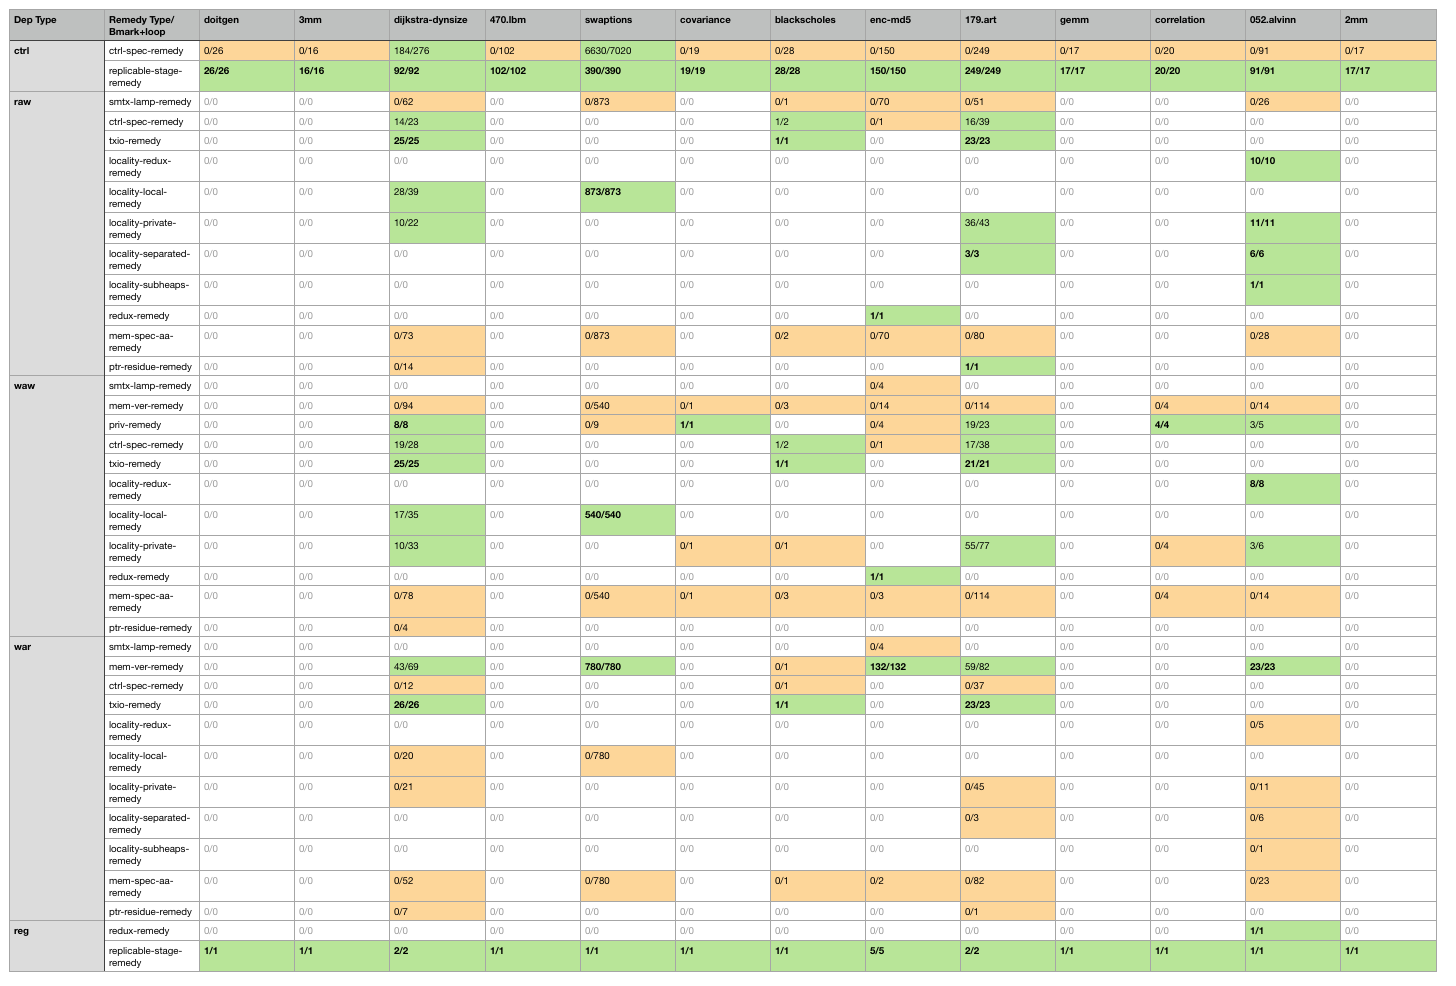
\includegraphics[width=\textwidth]{figures/table.png}
% \label{table:enabler-stats}


% \begin{table}[]
% \label{table:enabler-stats}
% \begin{tabular}{lllllllllllllll}

% Dep Type & Remedy Type/Bmark+loop    & doitgen & 3mm   & dijkstra-dynsize &
% 470.lbm & swaptions & covariance & blackscholes & enc-md5 & 179.art & gemm  &
% correlation & 052.alvinn & 2mm   \\

% ctrl     & ctrl-spec-remedy          & 0/26    & 0/16  & 184/276          &
% 0/102   & 6630/7020 & 0/19       & 0/28         & 0/150   & 0/249   & 0/17  &
% 0/20        & 0/91       & 0/17  \\

%          & replicable-stage-remedy   & 26/26   & 16/16 & 92/92            &
%          102/102 & 390/390   & 19/19      & 28/28        & 150/150 & 249/249 &
%          17/17 & 20/20       & 91/91      & 17/17 \\

% raw      & smtx-lamp-remedy          & 0/0     & 0/0   & 0/62             & 0/0
% & 0/873     & 0/0        & 0/1          & 0/70    & 0/51    & 0/0   & 0/0
% & 0/26       & 0/0   \\
%          & ctrl-spec-remedy          & 0/0     & 0/0   & 14/23            & 0/0
%          & 0/0       & 0/0        & 1/2          & 0/1     & 16/39   & 0/0   &
%          0/0         & 0/0        & 0/0   \\

%          & txio-remedy               & 0/0     & 0/0   & 25/25            & 0/0
%          & 0/0       & 0/0        & 1/1          & 0/0     & 23/23   & 0/0   &
%          0/0         & 0/0        & 0/0   \\

%          & locality-redux-remedy     & 0/0     & 0/0   & 0/0              & 0/0
%          & 0/0       & 0/0        & 0/0          & 0/0     & 0/0     & 0/0   &
%          0/0         & 10/10      & 0/0   \\

%          & locality-local-remedy     & 0/0     & 0/0   & 28/39            & 0/0
%          & 873/873   & 0/0        & 0/0          & 0/0     & 0/0     & 0/0   &
%          0/0         & 0/0        & 0/0   \\

%          & locality-private-remedy   & 0/0     & 0/0   & 10/22            & 0/0
%          & 0/0       & 0/0        & 0/0          & 0/0     & 36/43   & 0/0   &
%          0/0         & 11/11      & 0/0   \\

%          & locality-separated-remedy & 0/0     & 0/0   & 0/0              & 0/0
%          & 0/0       & 0/0        & 0/0          & 0/0     & 3/3     & 0/0   &
%          0/0         & 6/6        & 0/0   \\

%          & locality-subheaps-remedy  & 0/0     & 0/0   & 0/0              & 0/0
%          & 0/0       & 0/0        & 0/0          & 0/0     & 0/0     & 0/0   &
%          0/0         & 1/1        & 0/0   \\

%          & redux-remedy              & 0/0     & 0/0   & 0/0              & 0/0
%          & 0/0       & 0/0        & 0/0          & 1/1     & 0/0     & 0/0   &
%          0/0         & 0/0        & 0/0   \\

%          & mem-spec-aa-remedy        & 0/0     & 0/0   & 0/73             & 0/0
%          & 0/873     & 0/0        & 0/2          & 0/70    & 0/80    & 0/0   &
%          0/0         & 0/28       & 0/0   \\

%          & ptr-residue-remedy        & 0/0     & 0/0   & 0/14             & 0/0
%          & 0/0       & 0/0        & 0/0          & 0/0     & 1/1     & 0/0   &
%          0/0         & 0/0        & 0/0   \\

% waw      & smtx-lamp-remedy          & 0/0     & 0/0   & 0/0              & 0/0
% & 0/0       & 0/0        & 0/0          & 0/4     & 0/0     & 0/0   & 0/0
% & 0/0        & 0/0   \\

%          & mem-ver-remedy            & 0/0     & 0/0   & 0/94             & 0/0
%          & 0/540     & 0/1        & 0/3          & 0/14    & 0/114   & 0/0   &
%          0/4         & 0/14       & 0/0   \\

%          & priv-remedy               & 0/0     & 0/0   & 8/8              & 0/0
%          & 0/9       & 1/1        & 0/0          & 0/4     & 19/23   & 0/0   &
%          4/4         & 3/5        & 0/0   \\

%          & ctrl-spec-remedy          & 0/0     & 0/0   & 19/28            & 0/0
%          & 0/0       & 0/0        & 1/2          & 0/1     & 17/38   & 0/0   &
%          0/0         & 0/0        & 0/0   \\

%          & txio-remedy               & 0/0     & 0/0   & 25/25            & 0/0
%          & 0/0       & 0/0        & 1/1          & 0/0     & 21/21   & 0/0   &
%          0/0         & 0/0        & 0/0   \\

%          & locality-redux-remedy     & 0/0     & 0/0   & 0/0              & 0/0
%          & 0/0       & 0/0        & 0/0          & 0/0     & 0/0     & 0/0   &
%          0/0         & 8/8        & 0/0   \\

%          & locality-local-remedy     & 0/0     & 0/0   & 17/35            & 0/0
%          & 540/540   & 0/0        & 0/0          & 0/0     & 0/0     & 0/0   &
%          0/0         & 0/0        & 0/0   \\

%          & locality-private-remedy   & 0/0     & 0/0   & 10/33            & 0/0
%          & 0/0       & 0/1        & 0/1          & 0/0     & 55/77   & 0/0   &
%          0/4         & 3/6        & 0/0   \\

%          & redux-remedy              & 0/0     & 0/0   & 0/0              & 0/0
%          & 0/0       & 0/0        & 0/0          & 1/1     & 0/0     & 0/0   &
%          0/0         & 0/0        & 0/0   \\

%          & mem-spec-aa-remedy        & 0/0     & 0/0   & 0/78             & 0/0
%          & 0/540     & 0/1        & 0/3          & 0/3     & 0/114   & 0/0   &
%          0/4         & 0/14       & 0/0   \\

%          & ptr-residue-remedy        & 0/0     & 0/0   & 0/4              & 0/0
%          & 0/0       & 0/0        & 0/0          & 0/0     & 0/0     & 0/0   &
%          0/0         & 0/0        & 0/0   \\

% war      & smtx-lamp-remedy          & 0/0     & 0/0   & 0/0              & 0/0
% & 0/0       & 0/0        & 0/0          & 0/4     & 0/0     & 0/0   & 0/0
% & 0/0        & 0/0   \\

%          & mem-ver-remedy            & 0/0     & 0/0   & 43/69            & 0/0
%          & 780/780   & 0/0        & 0/1          & 132/132 & 59/82   & 0/0   &
%          0/0         & 23/23      & 0/0   \\

%          & ctrl-spec-remedy          & 0/0     & 0/0   & 0/12             & 0/0
%          & 0/0       & 0/0        & 0/1          & 0/0     & 0/37    & 0/0   &
%          0/0         & 0/0        & 0/0   \\

%          & txio-remedy               & 0/0     & 0/0   & 26/26            & 0/0
%          & 0/0       & 0/0        & 1/1          & 0/0     & 23/23   & 0/0   &
%          0/0         & 0/0        & 0/0   \\

%          & locality-redux-remedy     & 0/0     & 0/0   & 0/0              & 0/0
%          & 0/0       & 0/0        & 0/0          & 0/0     & 0/0     & 0/0   &
%          0/0         & 0/5        & 0/0   \\

%          & locality-local-remedy     & 0/0     & 0/0   & 0/20             & 0/0
%          & 0/780     & 0/0        & 0/0          & 0/0     & 0/0     & 0/0   &
%          0/0         & 0/0        & 0/0   \\

%          & locality-private-remedy   & 0/0     & 0/0   & 0/21             & 0/0
%          & 0/0       & 0/0        & 0/0          & 0/0     & 0/45    & 0/0   &
%          0/0         & 0/11       & 0/0   \\

%          & locality-separated-remedy & 0/0     & 0/0   & 0/0              & 0/0
%          & 0/0       & 0/0        & 0/0          & 0/0     & 0/3     & 0/0   &
%          0/0         & 0/6        & 0/0   \\

%          & locality-subheaps-remedy  & 0/0     & 0/0   & 0/0              & 0/0
%          & 0/0       & 0/0        & 0/0          & 0/0     & 0/0     & 0/0   &
%          0/0         & 0/1        & 0/0   \\

%          & mem-spec-aa-remedy        & 0/0     & 0/0   & 0/52             & 0/0
%          & 0/780     & 0/0        & 0/1          & 0/2     & 0/82    & 0/0   &
%          0/0         & 0/23       & 0/0   \\

%          & ptr-residue-remedy        & 0/0     & 0/0   & 0/7              & 0/0
%          & 0/0       & 0/0        & 0/0          & 0/0     & 0/1     & 0/0   &
%          0/0         & 0/0        & 0/0   \\

% reg      & redux-remedy              & 0/0     & 0/0   & 0/0              & 0/0
% & 0/0       & 0/0        & 0/0          & 0/0     & 0/0     & 0/0   & 0/0
% & 1/1        & 0/0   \\

%          & replicable-stage-remedy   & 1/1     & 1/1   & 2/2              & 1/1
%          & 1/1       & 1/1        & 1/1          & 5/5     & 2/2     & 1/1   &
%          1/1         & 1/1        & 1/1
% \end{tabular}
% \end{table}

% Discussion of the table


